\documentclass[../main/main.tex]{subfiles}
\begin{document}

\dominitoc
\faketableofcontents
\dominilof
\fakelistoffigures
\dominilot
\fakelistoftables

\chapter{Supernovae de type Ia}\label{ch:sne}

\epigraph{\openquote\ Il faut porter en soi un chaos pour pouvoir mettre
au monde une étoile dansante.\closequote}{\textsc{Nietzsche}, \textit{Ainsi
parlait Zarathoustra}}

Il existe toute une zoologie d'astres dans l'Univers, entre les planètes, les
étoiles, les galaxies… Mais ceux-ci étaient pendant longtemps considérés comme
immuables. C'est ainsi qu'en observant une nouvelle «~étoile~» dans le ciel en
1572, l'astronome Tycho \textsc{Brahé} la nomma \textit{nova}. Ça n'est qu'un
peu avant le milieu de XX\ieme~siècle que le terme «~supernova~» fut employé
pour la première fois par~\cite{baade1934}.

\vfill
\minitoc
\vfill
\newpage

\section{Fin de vie des étoiles}\label{sec:death}
\subsection{Classification}\label{ssec:class} % strolger2004, 2.2

\begin{figure}[ht]
    \centering
    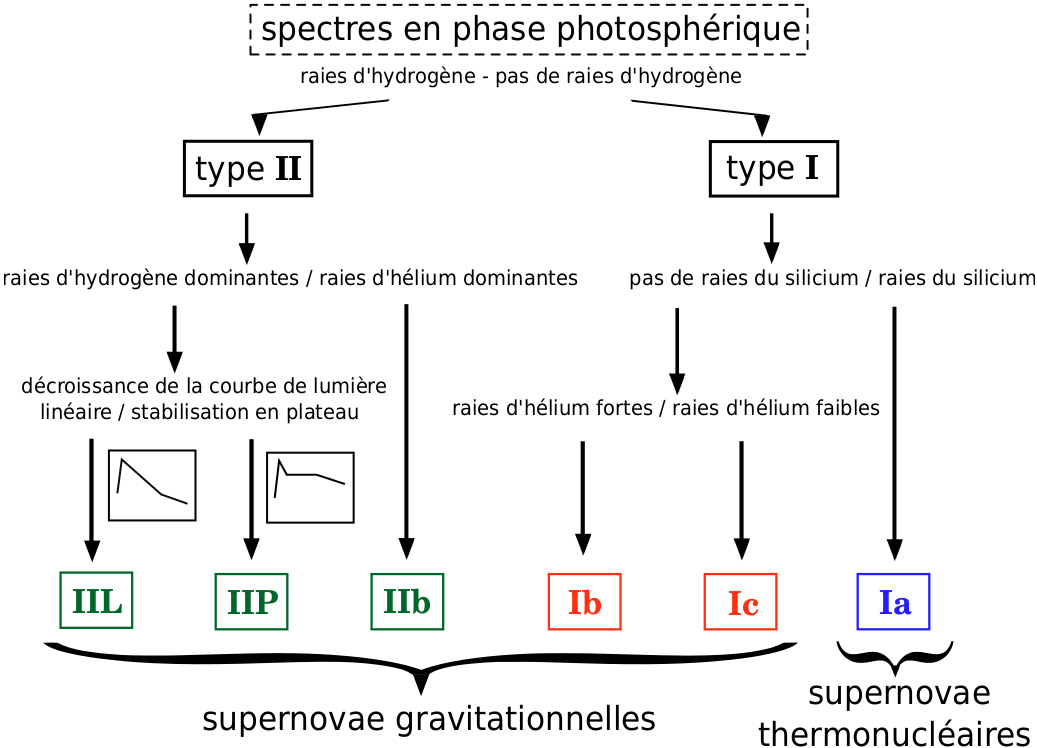
\includegraphics[width=.8\linewidth]{fourmanoit_sne}
    \caption[Classification des différents types de SNe selon leurs
    caractéristique spectrales]{Classification des différents types de SNe selon leurs
    caractéristique spectrales. Graphique tiré de la thèse
de~\cite{fourmanoit2010}.}\label{fig:sne_class}
\end{figure}

\subsection{Physique de l'explosion}\label{ssec:explo}

\section{Propriétés}\label{sec:sneprop}
\subsection{Courbe de lumière}\label{ssec:lc}
\subsubsection*{$t_0$}
\subsubsection*{$c$}
\subsubsection*{$x_0$}
\subsubsection*{$x_1$}
\subsection{Spectroscopie}\label{ssec:spectro}

\section{Standardisation}\label{sec:stand}
\subsection{Corrélations}\label{ssec:corr}
\subsection{Modèle \texttt{SALT2.4}}\label{ssec:salt}

\section{Cosmologie avec les SNe~Ia}\label{sec:snecosmo}
\subsection{Diagramme de Hubble}\label{ssec:hubble}
\subsection{Détermination des paramètres cosmologiques}\label{ssec:pcosmo}
\subsection{Biais actuels}\label{ssec:biais}

Pour ces raisons, on étudie l'évolution des SNe~Ia

\newpage

\thispagestyle{plain}
% \vspace*{-3cm}
\vfill
\minilof
\vfill
\minilot
\vfill

\bibliographystyle{../main/aa_url}
\shorthandoff{:}
\bibliography{../chapters/99_references}

\end{document}
